\documentclass{article}
\usepackage{graphicx}
\usepackage{float}

\title{Documentação do PI}
\author{Kauê José Abdalla Leal}
\date{16/04/2024}

\begin{document}

\maketitle

\begin{center}
Izabela Tayná Reis Coimbra (PO)\\
Kauê José Abdalla Leal (Design e Documentação)\\
Isabela Maria de Oliveira (Back-End)\\
Pedro Victor Virgino da Cunha (Front-End)\\
Victor Ferreira Neves (Front-End e Back-End)
\end{center}

\newpage

\begin{center}
\textbf{Documentação}
\end{center}


\section{Briefing}
Viajar, para muitos, é uma experiência transcendental, um momento de descoberta e aventura. No entanto, por trás da maravilha das paisagens exóticas e dos sorrisos em fotos, existe uma jornada de planejamento muitas vezes árdua e complexa. É nesse cenário desafiador que nasce nosso projeto: uma plataforma inovadora voltada para o planejamento de viagens, compartilhamento de experiências e dicas de economia.
Nossa história é moldada por diversos atores, cada um com seu papel único. Temos os viajantes individuais, sedentos por aventura e novas descobertas. Os grupos de viajantes, unidos pelo espírito de camaradagem e pela busca de experiências compartilhadas. E, é claro, nossa comunidade online de viajantes, o coração pulsante dessa jornada coletiva. O dilema é universal: escolher destinos, estimar custos, montar itinerários e enfrentar a barreira linguística são apenas alguns dos obstáculos que os viajantes enfrentam. Nosso propósito é simplificar essa jornada, oferecendo uma solução centralizada e confiável.
A jornada do viajante está repleta de desafios que demandam soluções digitais inteligentes. Desde o desenvolvimento de uma plataforma centralizada de planejamento de viagens até a agregação de informações confiáveis, cada etapa do processo é uma oportunidade para criar valor para nossa comunidade. Facilitar o compartilhamento de experiências, construir e manter uma comunidade global de viajantes e explorar oportunidades de monetização são áreas que exigirão foco e inovação para alcançar o sucesso. O coração do nosso projeto reside em uma plataforma online, meticulosamente desenvolvida para abrigar todas as necessidades do viajante moderno. Aqui, é possível pesquisar destinos, obter estimativas de custos, organizar itinerários e até mesmo facilitar a comunicação em terras estrangeiras. Tudo isso em um único lugar, com acesso fácil e intuitivo.
Nossa escolha pela área de negócio do turismo e viagens é respaldada por uma série de justificativas sólidas. A demanda crescente por soluções de planejamento de viagem acessíveis e confiáveis é evidente em um mundo onde viajar se torna cada vez mais acessível. O aumento do número de viajantes independentes e de baixo orçamento clama por uma plataforma que atenda às suas necessidades específicas. Além disso, reconhecemos a importância da comunidade e do compartilhamento de experiências na tomada de decisões de viagem, um aspecto que será fundamental em nosso projeto. E, por fim, a oportunidade de monetização através de parcerias e publicidade direcionada garante não apenas a sustentabilidade financeira da plataforma, mas também a entrega de valor adicional aos nossos usuários.

\section{Plano 5WH1}

\begin{enumerate}
      \item O que é o problema? (What)

            O processo de planejamento de viagem é complexo e desafiador para muitos viajantes. Eles enfrentam dificuldades ao escolher destinos, estimar custos, organizar itinerários e se comunicar em ambientes estrangeiros.
      \item Por que o problema ocorre? (Why)

            O problema ocorre devido à falta de acesso a informações confiáveis, dificuldade em compartilhar experiências de viagem e a necessidade de conectividade com uma comunidade global de viajantes.
      \item Quem são as pessoas que vivem o problema? (Who)

            Viajantes individuais, grupos de viajantes e a comunidade online de viajantes são os principais atores envolvidos.
      \item Onde as pessoas que vivem o problema estão? (Where)

            Os viajantes enfrentam esse problema em todas as etapas do processo de planejamento de viagens, desde a escolha do destino até a execução do itinerário em um ambiente estrangeiro.
      \item Quando o problema acontece? (When)

            O problema ocorre sempre que os viajantes estão planejando, organizando ou executando suas viagens, especialmente quando enfrentam dificuldades de logística, comunicação ou seleção de atividades.
      \item Como o problema acontece? (How)

            O problema surge devido à falta de acesso a informações confiáveis, à dificuldade de comunicação em ambientes estrangeiros e à ausência de uma comunidade online para compartilhar experiências e dicas.

\end{enumerate}

\section{Personas}

\begin{itemize}
      \item[$\bullet$] Viajantes Individuais
      \item[] Estes são indivíduos que buscam aventura e novas descobertas através de viagens.
            Eles podem ter diferentes faixas etárias, interesses e orçamentos, mas compartilham uma paixão por explorar o desconhecido.
            Suas necessidades incluem informações detalhadas sobre destinos, dicas de economia, itinerários personalizados e suporte durante a viagem.
      \item[$\bullet$] Grupos de Viajantes
      \item[] Este grupo é composto por amigos, famílias ou colegas que viajam juntos em busca de experiências compartilhadas e camaradagem.
            Eles podem precisar de recursos específicos para planejar viagens em grupo, como opções de hospedagem para grupos grandes, atividades adequadas para diferentes idades e preferências, e ferramentas para coordenar itinerários.
      \item[$\bullet$] Comunidade Online de Viajantes
      \item[] Esta é a comunidade virtual de usuários da plataforma, composta por viajantes individuais e grupos que interagem, compartilham experiências e dicas.
            Eles desempenham um papel crucial na geração de conteúdo gerado pelo usuário, fornecendo avaliações, recomendações e feedback.
            Sua participação é essencial para a construção de uma base de conhecimento confiável e atualizada sobre destinos, acomodações, atividades e muito mais.
      \item {\subsection {Outras Personas}}
      \item[] Hotéis
      \item[] Companhias Aéreas
      \item[] Agências de Turismo
      \item[] Anunciantes Interessados
\end{itemize}
{\subsection{Personagens}}
Viajante Individual:

- Identificação: Maria Silva, 32 anos, escritora freelancer apaixonada por viagens e culturas diversas.

- Objetivo: Maria busca constantemente inspiração para seus escritos através de novas experiências e lugares. Ela deseja explorar destinos autênticos, longe do turismo convencional, e compartilhar suas descobertas com seus leitores.

- Tarefas: Maria pesquisa intensamente sobre cada destino, procurando informações detalhadas sobre a cultura local, gastronomia, pontos turísticos menos conhecidos e meios de transporte acessíveis. Ela elabora itinerários personalizados, focados em experiências autênticas e imersivas.

- Dores e Frustrações: Maria muitas vezes se sente sobrecarregada com a quantidade de informações disponíveis e tem dificuldade em filtrar o que é relevante. Ela também enfrenta desafios ao tentar viajar com um orçamento limitado, especialmente quando se trata de encontrar hospedagem acessível em áreas menos turísticas.

- Possíveis Soluções: Maria poderia se beneficiar de uma plataforma que ofereça conteúdo detalhado e confiável sobre destinos, incluindo dicas de economia e sugestões de itinerários fora do comum. Um sistema de recomendação personalizado, baseado em suas preferências e interesses, poderia simplificar sua pesquisa. Além disso, acesso a uma comunidade online de viajantes onde ela possa trocar experiências e receber sugestões de outros viajantes individuais seria valioso para ela.

\bigskip
Grupo de Viajantes:

- Identificação: Família Santos, composta por João (pai), Ana (mãe), e seus dois filhos, Pedro (10 anos) e Sofia (7 anos).

- Objetivo: A família Santos procura criar memórias inesquecíveis juntos, explorando novos lugares e compartilhando experiências significativas. Eles buscam destinos que ofereçam uma variedade de atividades adequadas para diferentes idades, garantindo diversão para todos os membros da família.

- Tarefas: João e Ana pesquisam destinos familiares que ofereçam uma combinação de atrações culturais, recreativas e educacionais. Eles organizam atividades familiares, como visitas a museus, parques temáticos e trilhas naturais, e procuram opções de hospedagem que acomodem confortavelmente toda a família.

- Dores e Frustrações: A família Santos enfrenta desafios ao tentar equilibrar as preferências e interesses de todos os membros. Eles também podem ter dificuldade em encontrar acomodações espaçosas o suficiente para uma família grande, especialmente em destinos populares durante períodos de alta temporada.

- Possíveis Soluções: Uma plataforma que ofereça informações sobre destinos familiares, incluindo atividades recomendadas para diferentes faixas etárias, seria útil para a família Santos. Recursos que facilitem a coordenação de itinerários entre os membros da família, como listas compartilhadas e calendários integrados, também seriam bem-vindos. Além disso, opções de hospedagem que ofereçam quartos familiares ou apartamentos espaçosos seriam ideais para eles.

\bigskip
Comunidade Online de Viajantes:

- Identificação: Carlos Mendes, 28 anos, entusiasta de viagens e fotografia, ativo em várias comunidades online de viajantes.

- Objetivo: Carlos adora compartilhar suas experiências de viagem com os outros e receber insights e dicas de outros viajantes. Ele vê a comunidade online como uma fonte valiosa de conhecimento e inspiração para suas próximas aventuras.

- Tarefas: Carlos participa ativamente de fóruns de viagem, compartilhando relatos detalhados de suas viagens, recomendações de lugares para visitar, e dicas práticas para outros viajantes. Ele também lê avaliações e comentários de outros membros da comunidade sobre destinos, acomodações e atividades.

- Dores e Frustrações: Carlos pode se sentir sobrecarregado com a quantidade de informações disponíveis e pode ter dificuldade em discernir entre opiniões e recomendações confiáveis e menos confiáveis. Ele também pode ficar frustrado com a falta de interação genuína e engajamento em algumas comunidades online.

- Possíveis Soluções: Carlos poderia se beneficiar de uma plataforma que facilite a descoberta de conteúdo relevante e confiável, utilizando algoritmos de recomendação e sistemas de classificação de usuários. Recursos de filtragem avançada também seriam úteis para ele encontrar informações específicas sobre destinos, atividades ou tipos de hospedagem. Além disso, uma comunidade online que incentive a interação genuína e o engajamento entre os membros seria ideal para ele.

\section{Matriz CSD}
 {\subsection{Imagem}}

\begin{figure}[H]
      \centering
      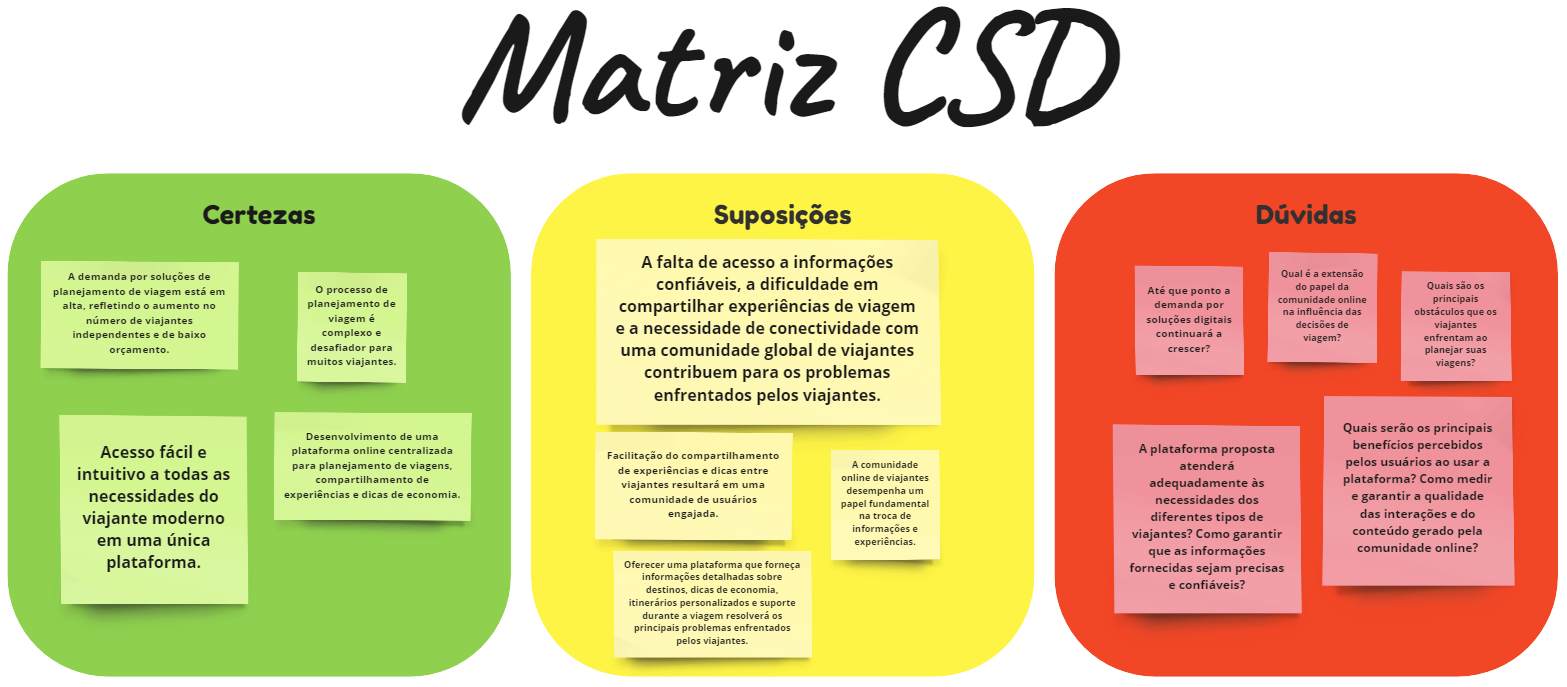
\includegraphics [width=1\textwidth]{IMGDOC/Matriz CSD.png}
      \label{csd imagem}
\end{figure}

{\subsection{Pesquisa com Google Forms / Pesquisa Quantitativa}}
Baseado na Matriz CSD, fizemos as seguintes perguntas para a pesquisa com o Forms:
\bigskip

O quanto você gosta de viajar?
\begin{figure}[H]
      \centering
      \includegraphics [width=1\textwidth]{IMGDOC/Quanto Gosta.png}
      \label{Pesquisa1}
\end{figure}

Quando você viaja, você posta nas redes sociais?
\begin{figure}[H]
      \centering
      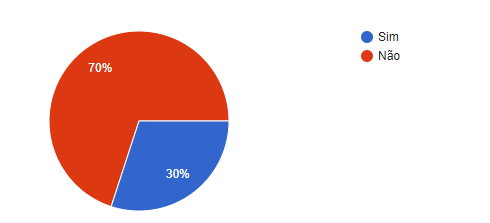
\includegraphics [width=1\textwidth]{IMGDOC/Redes sociais.png}
      \label{Pesquisa2}
\end{figure}

Você já teve dificuldades para planejar uma viagem?
\begin{figure}[H]
      \centering
      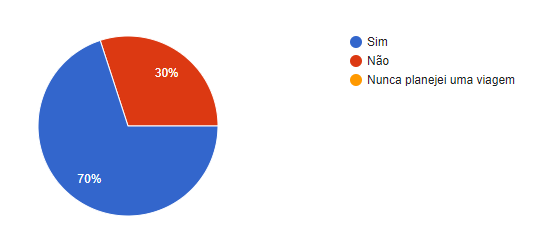
\includegraphics [width=1\textwidth]{IMGDOC/Dificuldades planejar.png}
      \label{Pesquisa3}
\end{figure}

Quando planejou a viagem, você demorou muito para planejar?
\begin{figure}[H]
      \centering
      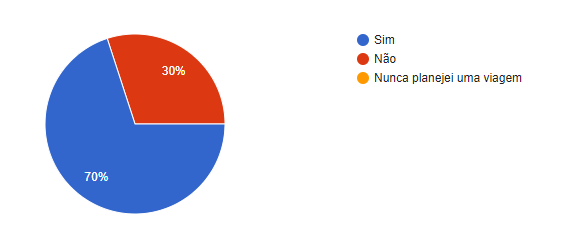
\includegraphics [width=1\textwidth]{IMGDOC/Demora planejar.png}
      \label{Pesquisa4}
\end{figure}

Você já teve muitas dificuldades para achar lugares baratos e confiáveis quando estava viajando?
\begin{figure}[H]
      \centering
      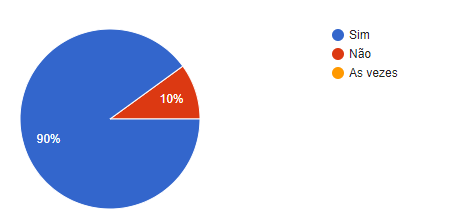
\includegraphics [width=1\textwidth]{IMGDOC/Dificuldades achar.png}
      \label{Pesquisa5}
\end{figure}

Baseado nas perguntas que você respondeu, você gostaria e acharia útil um site ou um app para uma comunidade de viajantes, feito para todos se ajudarem?
\begin{figure}[H]
      \centering
      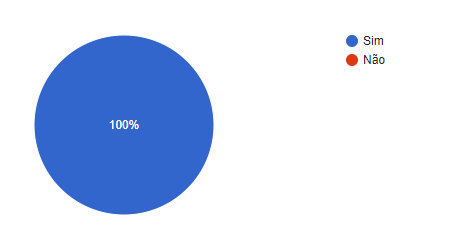
\includegraphics [width=1\textwidth]{IMGDOC/Fim pesquisa.png}
      \label{Pesquisa6}
\end{figure}

Algumas pessoas que participaram:
\begin{figure}[H]
      \centering
      \includegraphics [width=0.5\textwidth]{IMGDOC/participantes.png}
      \label{Pesquisa7}
\end{figure}


{\subsection{Entrevista / Pesquisa Qualitativa}}
Pesquisa feita no dia 15/04, às 15:36. Nome do participante: Kayk Cesar

Resumo:

"- Você gosta muito de viajar?"

"- Gosto bastante. Para mim, é uma das melhores experiências que podemos ter, explorar novos lugares e culturas."

"- Você já passou por algum desafio quando foi planejar alguma viagem?"

"- Sim, já tive algumas dificuldades ao planejar viagens. Às vezes, é complicado conciliar horários, encontrar acomodações adequadas e decidir quais atividades incluir no itinerário.
Já passei por algumas experiências em que eu não conseguia achar lugares baratos. Especialmente em destinos desconhecidos, pode ser difícil discernir entre opções que oferecem um bom custo-benefício e aqueles que são apenas uma armadilha para turistas."

"- Você acha que deveria ter algo para ajudar pessoas a não passar por essas dificuldades?"

" -Com base nas minhas experiências, acho que um site ou aplicativo para a comunidade de viajantes seria extremamente útil. Seria ótimo ter um espaço onde as pessoas possam compartilhar dicas, recomendações, experiências e até mesmo oferecer ajuda mútua durante o processo de planejamento de viagens."

\bigskip

\section{Benchmark}
De acordo com pesquisas feitas em sites e redes sociais, os concorrentes tem dificuldades em alguns aspectos, trivago e mochileiros.com não postam muito em suas redes sociais.
Trivago tem problemas com o desempenho de seus sites, já mochileiros.com tem problemas com o desempenho e com sua acessibilidade em seu site.

\subsection{Gráficos Trivago}

\begin{figure}[H]
      \centering
      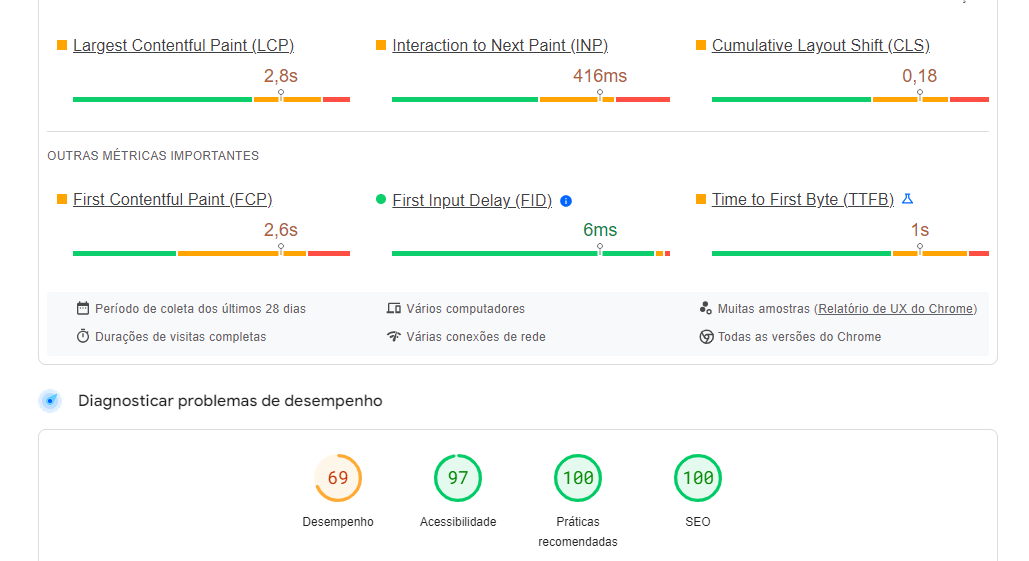
\includegraphics [width=1\textwidth]{IMGDOC/AnaliseTrivago1.png}
      \label{pesq1 tri}
\end{figure}
\begin{figure}[H]
      \centering
      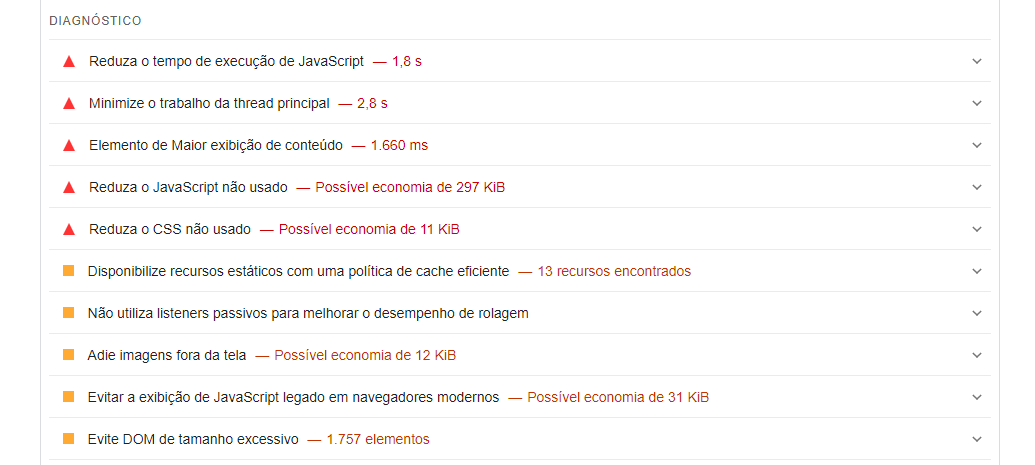
\includegraphics [width=1\textwidth]{IMGDOC/AnaliseTrivago2.png}
      \label{pesq2 tri}
\end{figure}

\subsection{Gráficos Mochileiros.com}

\begin{figure}[H]
      \centering
      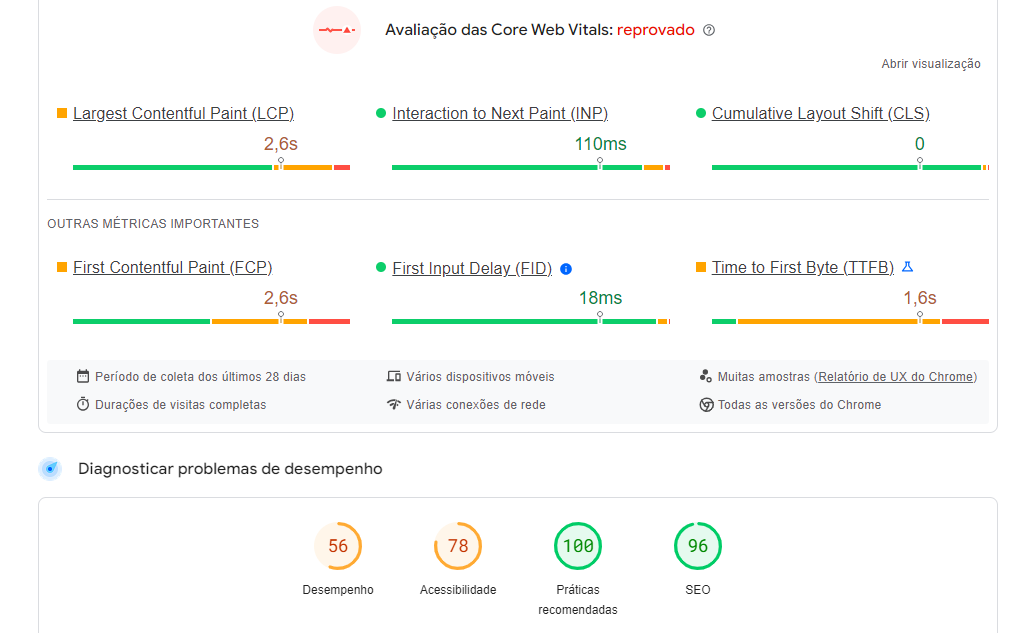
\includegraphics [width=1\textwidth]{IMGDOC/AnaliseMochileiros1.png}
      \label{pesq1 mochi}
\end{figure}
\begin{figure}[H]
      \centering
      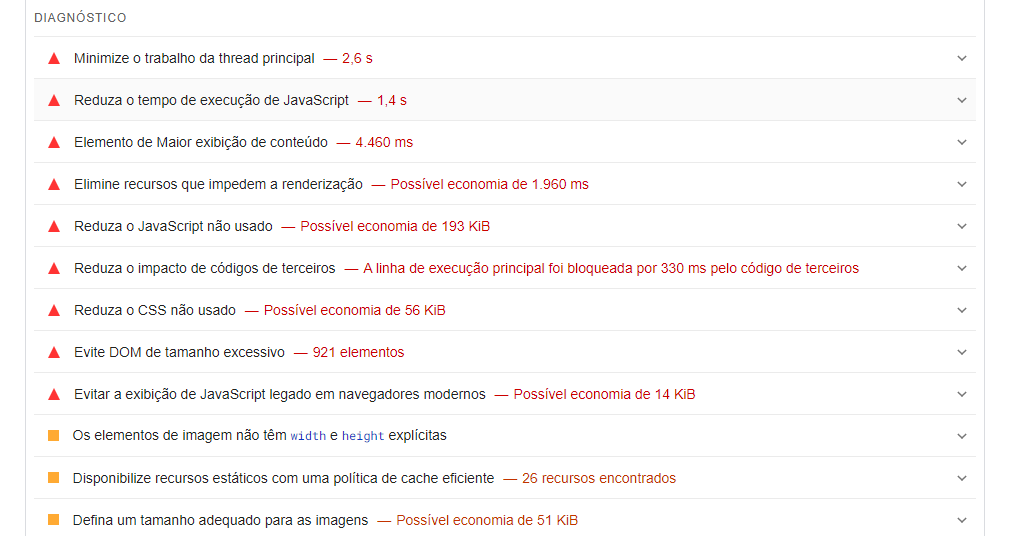
\includegraphics [width=1\textwidth]{IMGDOC/AnaliseMochileiros2.png}
      \label{pesq2 mochi}
\end{figure}

\section{Mapa da jornada do usuário}
\subsection{Sem a aplicação}

\begin{figure}[H]
      \centering
      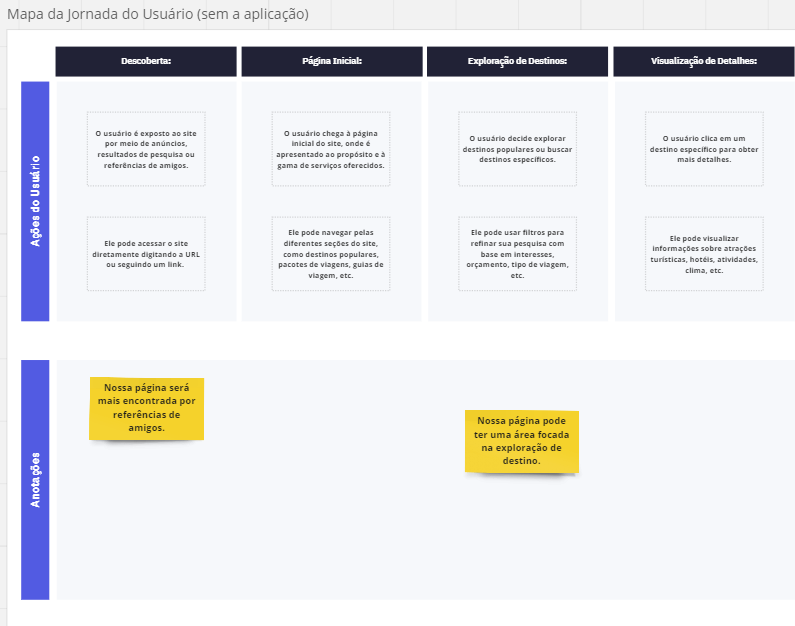
\includegraphics [width=1\textwidth]{IMGDOC/MapaSemA1.png}
      \label{mapa sem a1}
\end{figure}
\begin{figure}[H]
      \centering
      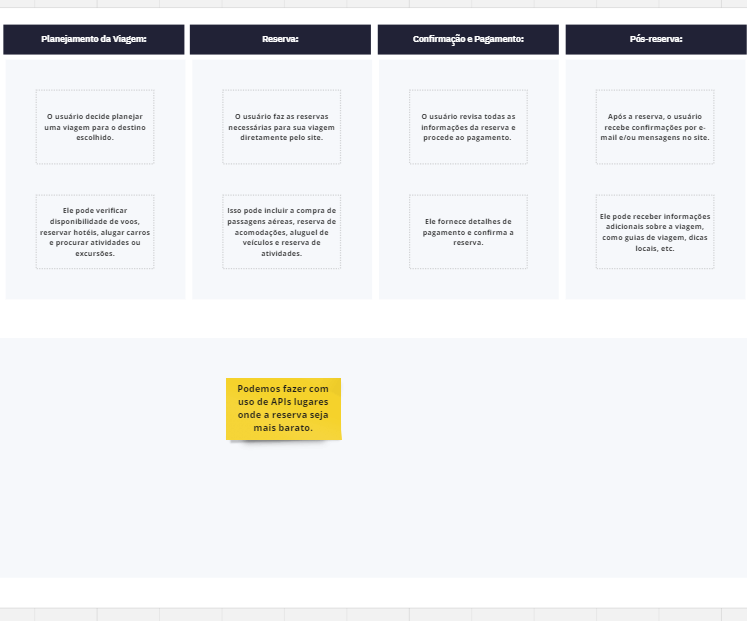
\includegraphics [width=1\textwidth]{IMGDOC/MapaSemA2.png}
      \label{mapa sem a2}
\end{figure}\begin{figure}[H]
      \centering
      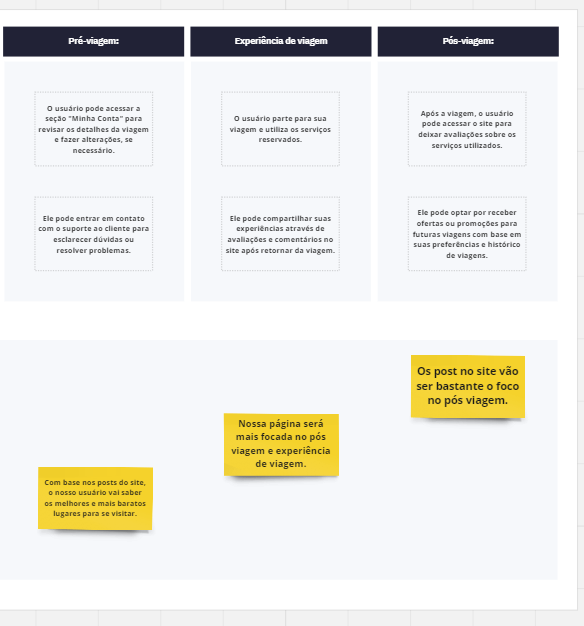
\includegraphics [width=1\textwidth]{IMGDOC/MapaSemA3.png}
      \label{mapa sem a3}
\end{figure}

\end{document}
